\section{Generation \& SiL testing of eFMUs}\label{sec:efmuGenAndSiL}

To generate eFMUs for the PSS and power system variants that have been designed and MiL-tested in Section \ref{sec:modeling-for-mil-testing}, Dymola offers the \texttt{DymolaEmbedded} library. It features a convenient user interface---graphical in the diagram and parameter editor views, yet also fully scriptable in \texttt{*.mos} files like any other Modelica library in Dymola---for configuring eFMU generation and conducting SiL tests of the resulting ISO/IEC 9899 (C11, C17, or C24 compliant) production code.

The production code of exported eFMUs leverages on the GALEC guarantees sketched in Section \ref{sec:efmi-standard}; in particular, Dymola's whole range of symbolic equation system optimizations are automatically conducted to find an algorithmic, inline-integrated eFMI GALEC solution for models subject to eFMU export.

\subsection{eFMU configurations}\label{sec:eFMU-configurations}

\begin{figure}[b!]
    \centerline{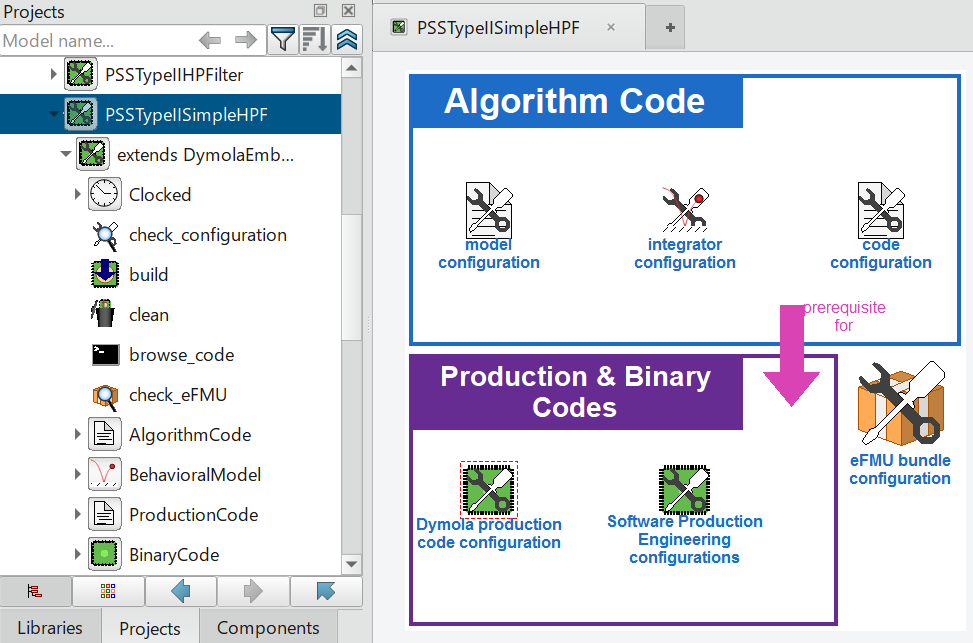
\includegraphics[width=0.99\columnwidth]{./figures/eFMU-configuration.png}}
    \vspace{-2ex}
    \caption{\texttt{DymolaEmbedded} eFMU configuration for the PSS \controller{} of Figure \ref{fig:pssvariants}~(D). Double-clicking on diagram-view components opens the respective configuration. Calling functions of the \textit{extends}-entry in the package browser executes the respective action, e.g., building GALEC or production code or analyzing code quality with clang-tidy or Cppcheck Premium.}
    \label{fig:eFMU-configuration}
    %\vspace{-4ex}
\end{figure}

To configure eFMU export for a Modelica model, a new package extending \texttt{DymolaEmbedded.EmbeddedConfiguration} has to be created. Each such extending-package represents an eFMU configuration and inherits configuration options and generative facilities as shown in Figure \ref{fig:eFMU-configuration}. The available configuration options are as follows:

\squishlist
    \item \textit{eFMU bundle configuration:} Optional name of the directory that shall contain the generated eFMU. If not explicitly set, the full qualified package name of the eFMU configuration is used.
    \item \textit{Model configuration:} Model subject to eFMU export (mandatory).
    \item \textit{Integrator configuration:} Fixed sampling period (mandatory) and optional solver method for inline-integration. The only mature solver currently supported is the explicit Euler method; implicit Euler and Rosenbrock methods~\cite{Olsson2017Rosenbrock} are still at the prototype stage for eFMU export.
    \item \textit{Code configuration:} Optional options to obfuscate generated GALEC code, constant-fold all parameters to reduce code size (parameters are hard-coded in the generated code rather than exposed through the GALEC block interface; dependent parameters are removed, preventing any later recalibration), and keep multi-dimensional entities intact rather than reducing them to scalars (e.g., used to preserve tensor-flows of embedded neural networks modeled using the \texttt{NeuralNetworks} package of the \texttt{eFMI} library, cf. \cite{Kamp2025}).
    \item \textit{Software Production Engineering configurations:} Preconfigured production code generator settings. Defines the floating-point precisions for which production codes shall be generated (by default for 32-bit and 64-bit)---these are the eFMU Production Code containers to generate. Also defines for which instruction set architectures (by default for x86, Microsoft\regtm{} Windows\regtm{} 32- and 64-bit) statically linked libraries shall be generated for each Production Code container---these are the eFMU Binary Code containers used for SiL simulation within Dymola (cf. Section \ref{sec:modelica-based-sil-tests}).
    \item \textit{Dymola production code configuration:} Deprecated embedded code export, predating Dymola's eFMI support.
\squishend

\noindent{}For the PSS and power system variants designed in Sections \ref{sec:pss-models} and \ref{sec:power-system-models}, an explicit Euler with a 0.2 ms sampling period is set as the integrator configuration. In addition, the \controller{} of Figure \ref{fig:pssvariants}~(D) and the \plant{} of Figure \ref{fig:g4chil} are chosen as model configurations, respectively. For both, code obfuscation is deactivated.

The generative facilities (i.e., inherited functions) provided by eFMU configurations are:

\squishlist
    \item \texttt{build()}: Generate eFMU with Algorithm, Production and Binary Code containers. Optionally also export SiL-stubs (cf. Section \ref{sec:modelica-based-sil-tests}) and source code FMUs for each generated Production Code container (cf. Section \ref{sec:production-code-export}). The root-level \texttt{build()} function exists for convenience; each eFMU container can be individually generated within the \texttt{build()} functions of the respective sub-packages (e.g., \texttt{ProductionCode.build()}).
    \item \texttt{browse\_code()}, \texttt{clean()}: Open the eFMU in the default file manager or shell (e.g., File Explorer and \texttt{cmd} in Microsoft Windows); delete all generated artifacts.
    \item \texttt{ProductionCode.check\_codes()}: Analyze Production Code containers with clang-tidy and Cppcheck Premium (cf. Section \ref{sec:production-code-quality-analyses}) for code quality and MISRA C:2023 compliance.
    \item \texttt{build\_FMUs()}, \texttt{build\_Simulink\_imports()}, and \texttt{build\_Arduino\_sketches()} of \texttt{ProductionCode}: Export Production Code containers as source code co-simulation FMUs, Simulink\regtm{} C Function blocks or Arduino\regtm{} sketches (cf. Section \ref{sec:production-code-export}), respectively.
    \item \texttt{BehavioralModel.build\_tests()}: Reuse existing Modelica experiments to derive SiL-tests for the production codes of the eFMU (cf. Section \ref{sec:modelica-based-sil-tests}).
\squishend

\noindent{}By default (i.e., if arguments are not interactively changed), the above generative eFMU facilities work with the options of their respective eFMU configuration (i.e., the \texttt{DymolaEmbedded.EmbeddedConfiguration} modifiers of their call context). Hence, it is not necessary to reconfigure eFMU export repeatedly when switching models or libraries; instead, configurations are stored together with their corresponding eFMU configuration package.

Note that being ordinary Modelica packages, eFMU configurations (their options and functions) can be scripted in Modelica \texttt{*.mos} scripts. This enables convenient configuration of variants and batch processing. Likewise, an \textit{eFMI}-button in Dymola's \textit{Tools}-ribbon (see Figure \ref{fig:eFMI-tools-ribbon-button}) enables the user to build all eFMUs of a whole package hierarchy, or load the SiL-stubs of existing eFMUs.

\begin{figure}[h!]%\centerline{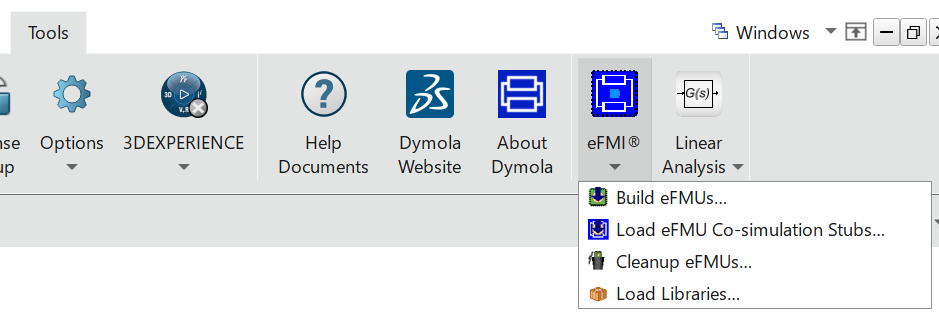
\includegraphics[width=0.95\columnwidth]{./figures/eFMI-tools-ribbon-button.png}}
\centerline{\includesvg[width=1.0\columnwidth]{./figures/eFMI-tools-ribbon-button.svg}}
    \vspace{-2ex}
    \caption{\textit{eFMI}-button in Dymola's \textit{Tools}-ribbon.}
    \label{fig:eFMI-tools-ribbon-button}
    \vspace{-2ex}
\end{figure}

\subsection{Modelica-based SiL tests}\label{sec:modelica-based-sil-tests}

\paragraph{SiL experiment packages:} To validate the functional correctness of the production codes generated for \controller{} and \plant{} models, we reused the MiL experiments of Section \ref{sec:mil-tests} as a basis to define respective SiL tests. To that end, Dymola's eFMI facilities support the generation of SiL experiment packages backed by an eFMI Behavioral Model container derived from an existing Modelica experiment; the \texttt{BehavioralModel.build\_tests()} function of an eFMU configuration (cf. Section \ref{sec:eFMU-configurations}) can be used to generate such SiL experiment packages. Given any Modelica experiment model, \texttt{build\_tests()} extracts---based on the \textit{model configuration} of the eFMU configuration in whose context it is executed---all instances of the model subject to eFMU code generation. Each instance defines a test scenario. 

\begin{figure}[t!]
    \centerline{\includesvg[width=1.0\columnwidth]{./figures/SiL-test-2.svg}}
    \vspace{-2ex}
    \caption{(A) SiL experiment package derived from the MiL experiment of Figure \ref{fig:refsim}, (B) SiL test model for the 32-bit floating-point precision production code generated for the PSS \controller{} of Figure \ref{fig:pssvariants}~(D).}
    \label{fig:SiL-test}
    \vspace{-2ex}
\end{figure}

Figure \ref{fig:SiL-test}~(A) shows the SiL experiment package (\texttt{SiLTest}) generated from the MiL experiment of Figure \ref{fig:refsim} for the \controller{} of Figure \ref{fig:pssvariants}~(D). The \texttt{Test\_ReferenceExperiment} model exploits the MiL experiment of Figure \ref{fig:refsim} to record reference trajectories. The \texttt{Test\_SiL\_} models are for testing the various production codes of the eFMU. The \texttt{build()} function simulates \texttt{Test\_ReferenceExperiment} and generates the Behavioral Model container backing the SiL experiment package, in particular its comma separated value (CSV) files with the reference trajectories and a manifest file with meta-information about the test scenarios, their in- and outputs, their respective units, etc. The \texttt{browse\_container()} function just opens the backing Behavioral Model container in the default file manager (e.g., File Explorer in Microsoft Windows).

\paragraph{SiL test models:} Figure \ref{fig:SiL-test}~(B) shows the SiL test model for the 32-bit floating-point precision production code for the \controller{} of Figure \ref{fig:pssvariants}~(D). The \texttt{eBlock} component is a SiL-stub generated for the production code. Such stubs are Modelica models with the same interface as the source model of an eFMU configuration, but their implementation is done by referencing the eFMU's production code by means of Modelica's external C code interface (the concept is similar to the Modelica stubs Dymola generates for imported FMUs). The \texttt{\textquotesingle{}vSI|table\textquotesingle{}} and \texttt{\textquotesingle{}vs|table\textquotesingle{}} components are input tables providing the reference trajectories for the PSS. The \texttt{\textquotesingle{}vs|match\textquotesingle{}} block simply compares the actual \texttt{vs} output of the production code (\texttt{eBlock.vs}) with the expected reference trajectory considering user-defined absolute and relative tolerances. The used tolerances can be defined for all scenarios, or specific ones, in the root diagram view of generated SiL experiment packages; they are the only additional user input required. Otherwise, the whole SiL experiment package can be generated from the MiL experiment of Figure \ref{fig:refsim}.

All components, except the \texttt{eBlock}, are from the \texttt{Testing}\footnote{\tiny{\url{https://www.youtube.com/watch?v=wnk5YbEgTjM}}} Modelica library, freely available with Dymola. \texttt{Testing} is a professional library to exploit Modelica experiments for testing purposes, automate regression tests (e.g., with Jenkins\footnote{\tiny{\url{https://www.jenkins.io/}}}), and provide convenient test results and plots. It is used for the continuous integration tests of the commercial Modelica library portfolio of Dassault Systèmes.

\paragraph{SiL test results:} The results of the SiL tests for our eFMUs are satisfactory. For the \controller{} of Figure \ref{fig:pssvariants}~(D), the \texttt{vs} output of the 32-bit floating-point precision production code has a maximum deviation of ${\approx}0.000365324$ for the test scenario of Figure \ref{fig:refsim} (note that the reference trajectories are recorded based on 64-bit floating-point precision simulations); the 64-bit production code has a maximum deviation of ${\approx}1.38778e-16$. The \texttt{w} output of the \plant{} of Figure \ref{fig:g4chil} has deviations as follows: ${\approx}0.000161166$ for 32-bit floating-point precision production code and ${\approx}-1.77636e-14$ for 64-bit.

Note that we will system integrate the 32-bit production codes in Section \ref{sec:STM32-integration-of-eFMUs} since the \controller{} STM32 board (NUCLEO-L476RG) supports hardware acceleration only for 32-bit floating-point precision and 64-bit floating-point precision production code for the \plant{} turned out to execute significantly slower on its STM32 board (NUCLEO-H723ZG) than the 32-bit floating-point precision code, leaving to little headroom with a very high risk of overruns in case of merely minor future model changes (cf. Section \ref{sec:results-and-analyses} for details).

\subsection{Production code quality analyses}\label{sec:production-code-quality-analyses}

To validate that eFMU production code generated by Dymola is of very high quality, Dymola provides preconfigured code quality checks with clang-tidy\footref{fnt:clang-tidy} and Cppcheck Premium\footref{fnt:cppcheck-premium}; the latter is particularly useful to validate MISRA C:2023 compliance. The preconfigurations are as verbose, complete and strict as possible.

\paragraph{Clang-tidy configuration:} For clang-tidy all checks are enabled except the following checks: (1) \textit{readability-identifier-length} (disabled because names of source Modelica models shall be reused, but in physics often very short variable names are used like \texttt{v} for voltage or \texttt{w} for rotational speed), (2) \textit{cppcoreguidelines-avoid-magic-numbers} and \textit{readability-magic-numbers} (physics equations can contain magic numbers), (3) \textit{altera-unroll-loops} and \textit{altera-id-dependent-backward-branch} (loop unrolling shall be done by the compiler, not the user; the implementation of multi-dimensional GALEC functions in generated production code is universal---their loops depend on the passed size arguments but these are literals at the call site, which is why we can assume compilers are capable of automatic optimization), and (4) \textit{altera-struct-pack-align} (code shall be portable and alignment automatically handled by the compiler).

\paragraph{Cppcheck Premium configuration:} For Cppcheck Premium the check-level is exhaustive, including style and information analyses; even inconclusive analyses are reported. Further MISRA C:2023 and SEI CERT C Coding Standard\footref{fnt:sei-cert-c} checks are enabled. For the implementation of GALEC built-in functions, a dedicated library configuration is provided to help Cppcheck identify built-in function API violations (e.g., if passed pointers to multidimensional variables must already be allocated and/or initialized).

\begin{figure*}[t]
    \centerline{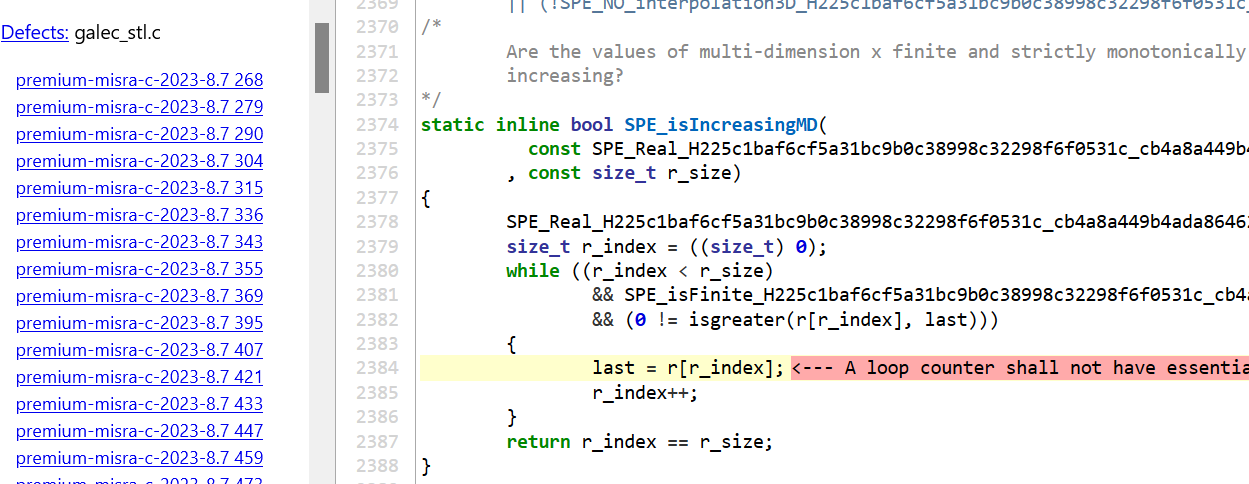
\includegraphics[width=1.5\columnwidth]{./figures/Cppcheck-report.png}}
    \vspace{-1ex}
    \caption{Excerpt of the Cppcheck Premium report for the 32-bit floating-point precision production code generated for the PSS \controller{} of Figure \ref{fig:pssvariants}~(D).}
    \label{fig:Cppcheck-report}
    \vspace{-2ex}
\end{figure*}

\paragraph{Code analyses results:} The results of the production code analyses for our examples can be found in the public repository\footref{fnt:pss-repository}; for each production code container in the \texttt{logs/check-code/clang-tidy} and \texttt{Cppcheck} subdirectories respectively. In the following discussion, we consider the 32-bit floating-point precision code for the \controller{} of Figure \ref{fig:pssvariants}~(D).

First of all, clang-tidy (Clang Tools 19.1.5) reports that 64-bit floating-point precision literals are assigned to 32-bit variables (\textit{bugprone-narrowing-conversions} and \textit{cppcoreguidelines-narrowing-conversions} violations); this is a shortcoming of Dymola's production code generator, which fails to add proper \texttt{F} suffixes, like in \texttt{1.0F / instance->wscale}. Note however, that the actual literals stem from the source model where they are in 64-bit precision. The narrowing when generating 32-bit floating-point precision production code is intended, but we fail to make it explicit to avoid  the reports. Further, clang-tidy reports that some local variables are not initialized (\textit{cppcoreguidelines-init-variables} violations), which, after manual inspection, are clearly false-positive reports. There are no further reports by clang-tidy.

The Cppcheck Premium 26.3.0 reports are much more interesting. They are syntax highlighted using Python Pygments\footnote{\tiny{\url{https://pygments.org/}}}, as shown in Figure \ref{fig:Cppcheck-report}. There are 204 reported issues, most are systematic false-positives considering our application. There are 159 violations of MISRA C:2023 Rule 8.7 (advisory), \textit{"Functions and objects should not be defined with external linkage if they are referenced in only one translation unit"}; all are about GALEC built-in functions, whose implementation is intended as shared library---hence, can be ignored. There are 23 violations of SEI CERT C DCL06-C, \textit{"Use meaningful symbolic constants to represent literal values"}; they stem from magic-numbers in physics equations---hence, can be ignored too. There are 3 violations of SEI CERT C INT30-C, \textit{"Ensure that unsigned integer operations do not wrap"}, which we know to be false-positives because the respective \texttt{index - 1} expressions can become at most 0 due to indexing starting at 1 in eFMI GALEC. All other reported issues fall into one of these categories, like a \texttt{typedef} or objects intended for library usage (MISRA C:2023 Rule 2.3 \& 8.9 (advisory) violations). The only interesting MISRA C:2023 violation reported is for Rule 14.1 (required), \textit{"A loop counter shall not have essentially floating type"}, which has been reported for a function deciding if an array only contains strictly increasing values (used to define an interpolation abscissa); this report is a false-positive the Cppcheck team meanwhile fixed in Cppcheck Premium 26.6.0 based on our findings.

\subsection{Production code export}\label{sec:production-code-export}

In general, Dymola-generated production code can be integrated into an embedded system with little effort, as will be illustrated for the STM32 ecosystem in Section~\ref{sec:stm32-system-integration-main-loop}. Nevertheless, Dymola supports dedicated production code export for popular embedded ecosystems. Export/import thereby means to use the C code of an eFMU Production Code container as is, add any required wrapper code and meta-information to satisfy target ecosystem API requirements, and import the code such that the further (in particular compilation) infrastructure of the target ecosystem can be used for system integration on actual hardware. Dymola supports export of production code for (the respective eFMU configuration facilities are listed in Section~\ref{sec:eFMU-configurations}):

\squishlist
    \item \textit{FMI\regtm{}:} Export as FMI\footref{fnt:fmi} 3.0 source code co-simulation FMU with \texttt{fixedInternalStepSize}. The only code added to exported production code, besides the mandatory \texttt{modelDescription.xml}, is the required implementation of \texttt{fmi3Functions.h}, which is lean, avoiding as much overhead of the generic FMI interface as possible while at the same time introducing sanity checks to ensure the FMU is used as intended (in particular called with its fixed sampling period or a proper multiple thereof). eFMU production code exported as source code FMU enables the use of eFMI on many dedicated real-time platforms with source code FMU import; the tooling of such platforms will take care of compiling and deploying the production code. Examples are ConfigurationDesk\regtm{} (dSPACE), TwinCAT\regtm{} (Beckhoff\regtm{}), or Silver\regtm{} (Synopsys\regtm{}).
    
    It is noteworthy that the eFMU production code based FMUs exported by Dymola are significantly smaller than FMUs exported with its normal source and binary code co-simulation FMU export. For the \controller{} of Figure \ref{fig:pssvariants}~(D) the eFMU production code backed source code FMU is ${\approx}31$ kB, its compiled binary code version for Microsoft Windows 11 64-bit on Intel\regtm{} x86-64 is ${\approx}176$ kB, whereas the model directly exported as source code FMU is ${\approx}5.41$ MB and binary code FMU is ${\approx}2.84$ MB (in both cases exported with protected variables excluded, only black box, FMI 3.0 co-simulation, and inline integration method explicit Euler). Likewise for the \plant{} of Figure \ref{fig:g4chil}: ${\approx}38$ kB for the eFMU backed source code FMU, ${\approx}220$ kB for the eFMU backed binary code FMU, ${\approx}5.49$ MB for the normal source code FMU, and ${\approx}2.93$ MB for the normal binary FMU.
    \item \textit{Simulink:} Generate a MATLAB\regtm{} script, that when executed on a Simulink C Function block instantiates it to execute the respective production code. The GALEC block-interface (and therefore in-, outputs and parameters of the production code) are properly typed with native Simulink embedded real-time target (ERT) types such that unnecessary type conversions can be avoided; as is any copying of multidimensions. The resulting block can be used, and combined in Simulink like any other block. ERT code generators will take care of proper system integration of the C Function block, but otherwise use its backing eFMU production code as is (i.e., skip code generation for it).
    \item \textit{Arduino:} Exports production code as Arduino sketch, adding the required \texttt{*.ino} file with initialization and main loop as well as commented code where to access inputs, outputs, and parameters. Exported sketches are ready for further development and deployment via the Arduino IDE, or any other Arduino compatible tooling.
\squishend

\noindent{}For all export/import options the high-quality standards of eFMU production code as generated by Dymola are preserved, including being free of additional library dependencies besides common C Standard Library routines (mostly \texttt{math.h}).
